\section{State of the Art for Discontinuous Galerkin Methods} % for the \MA equation}

The most natural attempt for a formulation of a DG method is to exploit the equations
\begin{align}
	\int_{\Omega} \mydet {D^2 u} v = \int_\Omega fv \qquad \text{ for all test functions } v. \label{eq: naiv ansatz}
\end{align}

In 2008 B\"ohmer investigated this ansatz for $C^1$ elements in \cite{Boehmer2008}. He derives a general $C^1$ method including statements on its stability and consistency. He is able to reduce the convergence analysis to the linearised case \cite[Section 9]{Boehmer2008}, and discovers that the weak and strong linear operators even coincide for his ansatz spaces meaning the diagram in figure \ref{fig: fe diagram} taken from \cite[Fig 2.2]{FGN2013} commutes.

\begin{figure}[H]
			\begin{center}
		\usetikzlibrary{matrix}

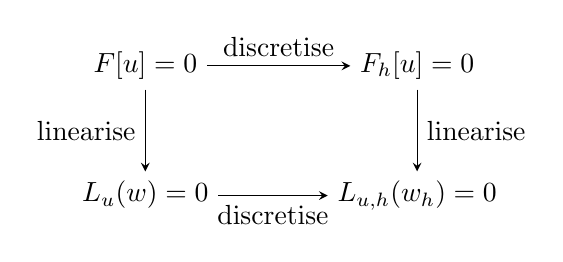
\begin{tikzpicture}[scale =2]
  \matrix (m) [matrix of math nodes,row sep=3em,column sep=4em,minimum width=2em]
  {
     F[u]=0 & F_h[u] =0 \\
     L_u(w) =0 & L_{u,h}(w_h)=0 \\};
  \path[-stealth]
    (m-1-1) edge node [left] {linearise} (m-2-1)
            edge node [above] {discretise} (m-1-2)
    (m-2-1.east|-m-2-2) edge node [below] {discretise} (m-2-2)
    (m-1-2) edge node [right] {linearise} (m-2-2);
\end{tikzpicture}
		\end{center}

	\label{fig: fe diagram}
	\caption{An abstract commuting diagram about the relation between weak and strong linear operators.\\ The analytical \MA operator is hereby denoted by $F:=\detHess u$ and its linearisation $L_u(w) = -\nabla \cdot (\cofHess u \nabla w)$, compare \ref{sec: linearisation}. $F_h[u]=0$ denots the discretised formulation, for B\"ohmer's method this is given by \eqref{eq: naiv ansatz}}.
\end{figure}

However, this formulation has two major disadvantages. 
At first we cannot throw the high derivatives onto the test functions using integration py parts, thus we do not cannot easily solve the arising system of equations. Secondly \eqref{eq: naiv ansatz} seems to work only for test and ansatz functions contained in $C^1(\Omega)$ whereas usual finite elements are contained in $C^0$. Brenner et alter make the inconsistency between the linearisation of the discrete problem and the the linearisation of the continuous problem, figuratively the non commutating of the diagram in figure \ref{fig: fe diagram} for less regular spaces,  responsible\cite{BGN+2011}. Their idea is to improve the discretised formulation by adding DG terms to force consistency and add stability.

\subsection{A $C^0$ Penalty Method }

Given zero boundary conditions the linearisation of the left-hand side of \eqref{eq: naiv ansatz} can be derived exactly as in the proof of theorem \ref{thm: linearisation} leading to the bilinear form
\begin{align}
\langle L_{u,h}(w_h),v_h\rangle =& \int_{\Omega} \nabla \cdot \left( \mycof {D^2 u_h } \nabla w_h \right) v_h
%=& \int_{\Omega} \left( \mycof {D^2 u_h } \nabla w_h \right) \nabla v_h. 
\label{eq: linearOperator}
\end{align}

Now we analyse the variational form of the linearisation of the \MA equation. Due to integration by parts it holds
\begin{align*}
  \int_T \nabla \cdot (\mycof{D^2 u_h} \nabla w_h) v_h= -\int_T (\mycof{D^2 u_h} \nabla w_h) \nabla v_h+ \int_{\partial T} (\mycof{D^2 u_h} \nabla w_h) v_h.
\end{align*}
Summing over the whole triangulation it becomes
\begin{align*}
  \int_\Omega \nabla \cdot (\mycof{D^2 u_h} \nabla w_h) v_h= -\int_\Omega (\mycof{D^2 u_h} \nabla w_h) \nabla v_h+ \sum_{e \in \edgesi} \int_{e} \llbracket \{\{\mycof{D^2 u_h} \}\} \nabla w_h\rrbracket v_h.
\end{align*}
Considering the last identity the variational form of the linearisation reads
\begin{align}
	\langle L^L_{u,h}(w_h),v_h\rangle 
	    =&- \sum_{T \in \triang}  \int_T \nabla \cdot (\mycof{D^2 u_h} \nabla w_h) v_h
	    + \sum_{e \in \edges} \int_{e} \llbracket \{\{\mycof{D^2 u_h} \}\} \nabla w_h\rrbracket v_h \nonumber \\
	    &+ \sum_{e \in \edges} \int_{e} \llbracket \{\{\mycof{D^2 u_h} \}\} \nabla v_h\rrbracket w_h \label{eq: var of linearisation}
\end{align}
Plugging the terms missing in \eqref{eq: linearOperator} but appearing in \eqref{eq: var of linearisation} into the original naive ansatz \eqref{eq: naiv ansatz} and adding further terms to enforce weak boundary conditions they formulate the problem: Find $u_h \in V_h$ such that
\begin{align}
\begin{split}
	&\int_{\Omega} (f-\mydet {D^2_h u_h} v 
	+ \sum_{e \in \edgesi} \int_{e} \llbracket \{\{\mycof{D^2 u_h} \}\} \nabla u_h\rrbracket v_h \\
	&- \sum_{e \in \edgesb} \int_{e} \llbracket \{\{\mycof{D^2 u_h} \}\} \nabla v_h\rrbracket (u_h -g) 
	+ \sigma  \sum_{e \in \edgesb} \frac 1 {h_e} \int_{e} (u_h -g)  = 0 \; \forall v_h \in V_h \label{eq: brenner method}
\end{split}
\end{align}
They choose their ansatz and test space $V_h$ to be the space of continuous functionous being piecewise polynomials up to degree $k$ for a $k \geq 3$. For these degrees and the case of classical solutions they provide a detailed analysis consisting of a proof of well-posedness and some error estimates. Their numerical results suggest optimal convergence rates \todo{convergence rates} for smooth solutions although they cannot confirm those with theoretical evidence. \\
However, their approach has a drawback. In order to find $u_h$ one has to solve the from \eqref{eq: brenner method} resulting nonlinear system. Brenner et alt. make use of Newton's method in the numerical results to solve their example problems. For a good initial guess they inquire a vanishing moments method which internally again solves nonlinear systems based on a Newton's method which uses a nested iteration to create initial guesses. 

We implemented their presented method using the finite element tool FEniCS \cite{FEniCS} and experienced a huge sensitivity for initial starting points. \todo{brauchen ja auch vanishing moments als start}
\todo{tolle numerische ergebnisse}

Neilan claims when presenting his method in \cite{Neilan2014} that this methods fails to converge for the test case
$u = -\sqrt{2 - x_1^2 - x_2^2 }$ and $f = \frac 2 {{2 - x_1^2 - x_2^2}^2}$ which lacks $H^2$ regularity, see also test \ref{test sqrt}. Generally the presented method is more appropriate for classical solutions, Brenner et alt. say they plan to address less regular solution in future work.


\subsection{A Finite Element Method based on a Discrete Hessian} \label{subsec: disrete Hessian} \label{sec: FEM discrete Hessian}

Shortly Neilan generalised in \cite{Neilan2014} a finite element method of Lakkis and Pryer presented in \cite{LP2011}.
The crux of this idea is the notion of a \emph{discrete Hessian}. 
While the real Hessian fulfills due to integration by parts as we have seen in Lemma \ref{la: integration by parts Frobenius}
	\begin{align}
		\int_\Omega (D^2 u : B) = - \int_\Omega \left(\nabla \cdot B\right) \cdot \nabla u + \int_{\partial \Omega}  B \nabla u \mathbf {n} \qquad \forall B \in [H^1(\Omega)]^{d \times d}, \label{eq: part int hessian}
	\end{align}
often the piecewise derived Hessian $D_h^2 v$ of $ v \in V_h$ for less regular ansatz spaces $V_h$ does not inherit this property. Considering that most weak formulations base on a integration by parts approach, the idea of a discretisation of the Hessian retaining this quality is standing to reason. To create this discretisation Neilan carries the integration from \eqref{eq: part int hessian} piecewise on every triangle out and rewrites the edge terms by a combination of jump and averages as usual leading to
	\begin{align}
		\begin{split}
		\int_\Omega (D^2 u : B) 
		=& - \int_\Omega \left(\nabla \cdot B\right) \cdot \nabla u \\
		&+ \sum_{ e \in \edgesi} \int_e  \jump {\average B \nabla u }
				+ \sum_{ e \in \edges} \int_e  \jump{B \average {\nabla u} }  \qquad \forall B \in \Sigma_h. \label{eq: part int hessian omega}
		\end{split}
	\end{align}
Observing, that the last step admits test functions $B$ only piecewise smooth, Neilan suggests the ansatz space $V_h = \mathcal{P}_h^k \cap H^1(\Omega)$ and the test space $\Sigma_h = [\mathcal{P}_h^k]^{d \times d}$.

Substituting in \eqref{eq: part int hessian omega} $\nabla u$ across the edges with its numerical counterpart, namely the numerical trace chosen as $\laverage \nabla u \raverage$ one has as predefinition of the discrete Hessian
\todo{lifting erwaehnen?}
	\begin{align}
		\int_\Omega (D_{DH}^2 u : B) 
		&= - \int_\Omega \left(\nabla \cdot B\right) \cdot \nabla u
		+ \sum_{ e \in \edgesi} \int_e  \jump {\average B \nabla u } 
				+ \sum_{ e \in \edges} \int_e \jump {B \average {\nabla u} }  \nonumber \\
		&= - \int_\Omega \left(\nabla \cdot B\right) \cdot \nabla u
				+ \sum_{ e \in \edges} \int_e  \jump{B \average {\nabla u} }.	
	\end{align}
Applying once more integration by parts for a Frobenius product on every triangle in the right-hande side integral results in
	\begin{align}
		\int_\Omega (D_{DH}^2 u : B) 
		=& \int_\Omega D_h u: B 
			-\sum_{ e \in \edgesi} \int_e  \jump {\average B  \nabla u }
			- \sum_{ e \in \edges} \int_e \jump {B \average {\nabla u} }\nonumber \\		
			&+ \sum_{ e \in \edges} \int_e  \jump {B \average {\nabla u} }		\nonumber \\
		=& \int_\Omega D_h u: B -\sum_{ e \in \edgesi} \int_e  \jump {\average B  \nabla u }				
	\end{align}

Hence,
\begin{definition}[Discrete Hessian]
	The discrete Hessian $D_{DH}^2 u$ of a function $u$ is the unique function satisfying
	\begin{align}
		\int_\Omega (D_{DH}^2 u : B) 
		= \int_\Omega D_h u: B -\sum_{ e \in \edgesi} \int_e  \jump {\average B \nabla u }\qquad \forall B \in \Sigma_h. \label{eq: discrete hessian}
	\end{align}
\end{definition}

Even though the Hessian is symmetric, in general the discrete Hessian is owing to the face terms not obligatory symmetric. \\
Note, that for a discontinuous $\Sigma_h$ the computations for $D_{DH}^2 u$ reduce to purely local efforts. For piecewise constant space $\Sigma_h$ the discrete Hessian $D_{DH}^2 u$ can even be computed explicitly.

The next natural step is to plug the newly deduced Hessian into the original \MA PDE resulting in the method: Find $u \in V_h$ such that

\begin{align}
		\int_\Omega \left(\mydet{D_{DH}^2 u} - f \right) v = 0 \qquad \forall v \in V_h \label{eq: neilan eq1}
\end{align}
where
	\begin{align}
		\int_\Omega (D_{DH}^2 u : B) 
		= \int_\Omega D_h u: B -\sum_{ e \in \edgesi} \int_e  \jump {\average B \nabla u }\qquad \forall B \in \Sigma_h. \tag{\ref{eq: discrete hessian}}
	\end{align}

Neilan shows the well-posedness and optimal error estimates of this methods for $k \geq 3$ in case the solution lies in $H^2(\Omega)$. Albeit he cannot prove it his numerical experiments suggest that it even works for smaller polynomial degrees and problems which's solution lacks $H^2$ regularity. Although for $k=1$ he adds an additional penalty term forcing thereby a smooth gradient to obtain convergence. Thus, he instead solves:
\begin{align}
		\int_\Omega \left(\mydet{D_{DH}^2 u} - f \right) v + \eta \sum_{e \in \edgesi} |e| \int_e \jump{ \nabla u_h} \jump{\nabla v}
		= 0 \qquad \forall v \in V_h \label{eq: neilan eq1 + jump}
\end{align}
where
	\begin{align*}
		\int_\Omega (D_{DH}^2 u : B) 
		= \int_\Omega D_h u: B -\sum_{ e \in \edgesi} \int_e  \jump {\average B \nabla u }\qquad \forall B \in \Sigma_h \tag{\ref{eq: discrete hessian}}
	\end{align*}
and $\eta$ is an additional penalty parameter which Neilan takes to be 50 in his numerical tests.

He does not present any proofs for convergence rates, but in the numerical results his method performs with optimal convergence rates. We check the performance of this algorithms later in chapter \ref{ch:NumericalResults}.